\documentclass[Rapport/Rapport_main.tex]{subfiles}
\begin{document}
\subsection{Controller-BallDispenserApp}
\subsubsection{Softwaredesign}
Denne komponenten er hoved kontrollen til ballDispenser, den er ansvarlig for styringen af både coinDispenser og ballDispenser. Den indeholder også funktionene som kreves får å sende og motta beskjeder til RPi. Dens hoved funksjon er coinInserted den kan sees under (Listing \ref{lst:dispenserControlFunction}). 
\begin{lstlisting}[caption={Hoved kontrol funksjonen til ballDispenser},style=customc,label={lst:dispenserControlFunction}]
void coinInserted()
{
    handleCoinDetection();
    if(countBalls() <= 2)
    {
        disableDispenser(); 
        sendDispenserStatus();
    }
    sendCoinDetected();
    dispenseBalls();
    resetDetectionISR();
}
\end{lstlisting}

For å opprette kommunikasjonen mellom BallDispenser og RPi brukes I2C slave modulet som er et modul fra PSoC Creator og et interrupt som trekkes lavt når BallDispenser har en Message som skal sendes til RPi.
\begin{figure}[H]
    \centering
    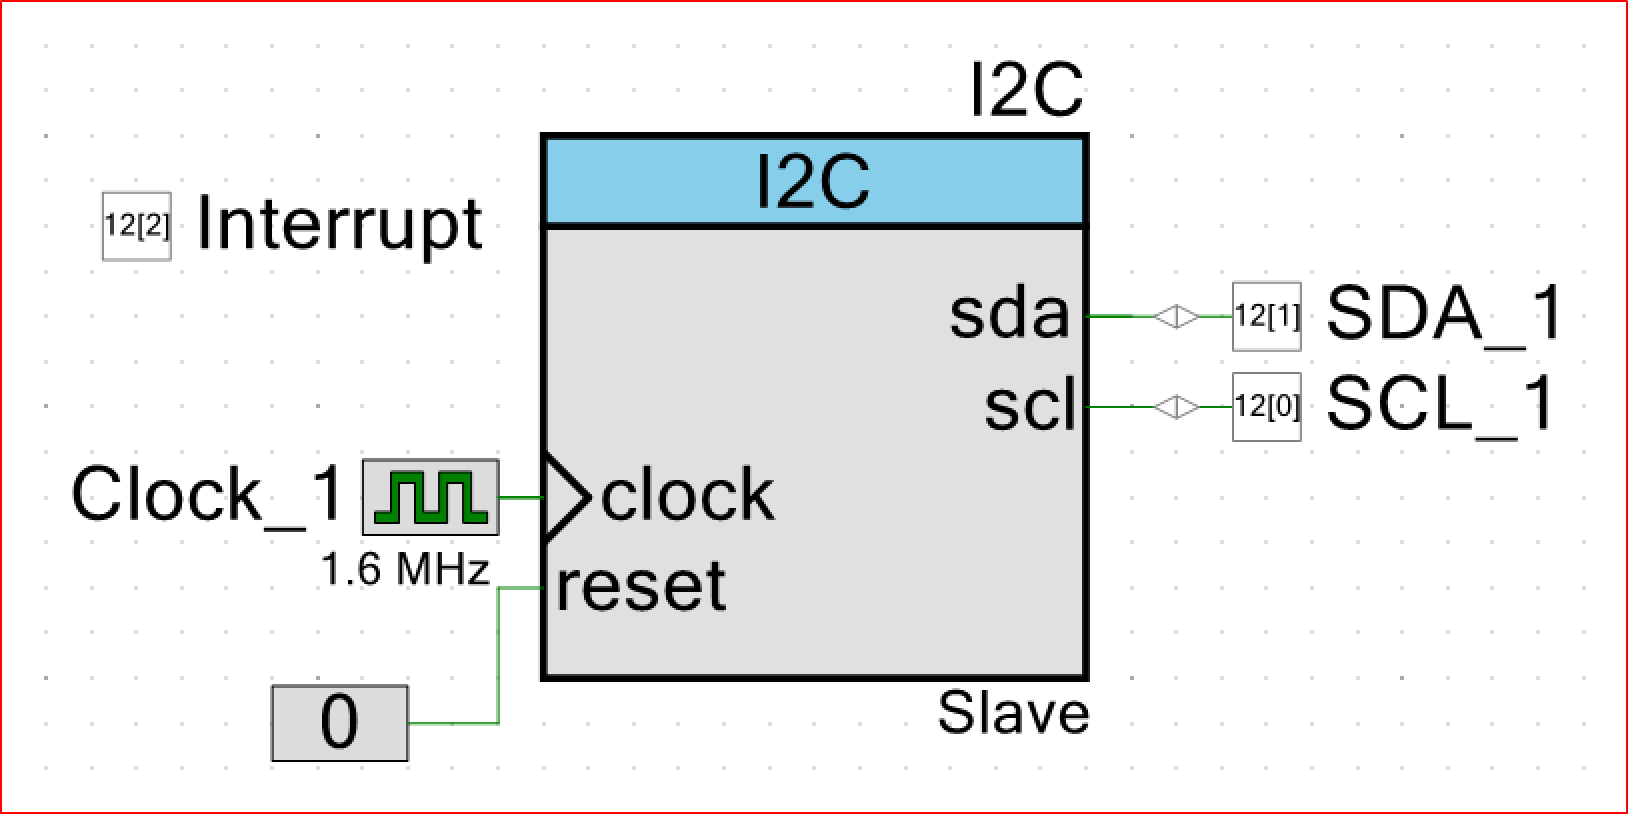
\includegraphics[width=\textwidth]{Rapport/BallDispenser/ballDispenserController/graphics/I2Cslave.png}
    \caption{I2C slave modul}
    \label{fig:I2CSlaveBallDisp}
\end{figure}

\subsubsection{Implementering}
Implementeringen av CoinDispenser er skrevet i  PSoC Creator som er utviklings plattformen til PSoC. Dokumentasjon kan sees i \textbf{Softwaredesign} dokumentet, avsnitt \fullref{swdesign:sec:BallDispController}
\subsubsection{Modul Test}
For modultest og resultater refereres det til \textbf{Modul Test} dokumentet, avsnitt \fullref{modultest:sec:DispController}
\end{document}